\documentclass{beamer}
\usetheme{Pittsburgh}
\usecolortheme{rose}

\usepackage{amsmath}
\usepackage{fancyvrb}
\usepackage[brazilian]{babel}
\usepackage[utf8]{inputenc}
\usepackage[T1]{fontenc}

\title{Problema da Mochila Binária}
\author{Fernando Gomes, Leonardo Holtz}
\institute{Universidade Federal do Rio Grande do Sul}
\date{}

\begin{document}

\begin{frame}

\titlepage

\begin{figure}
    \centering
    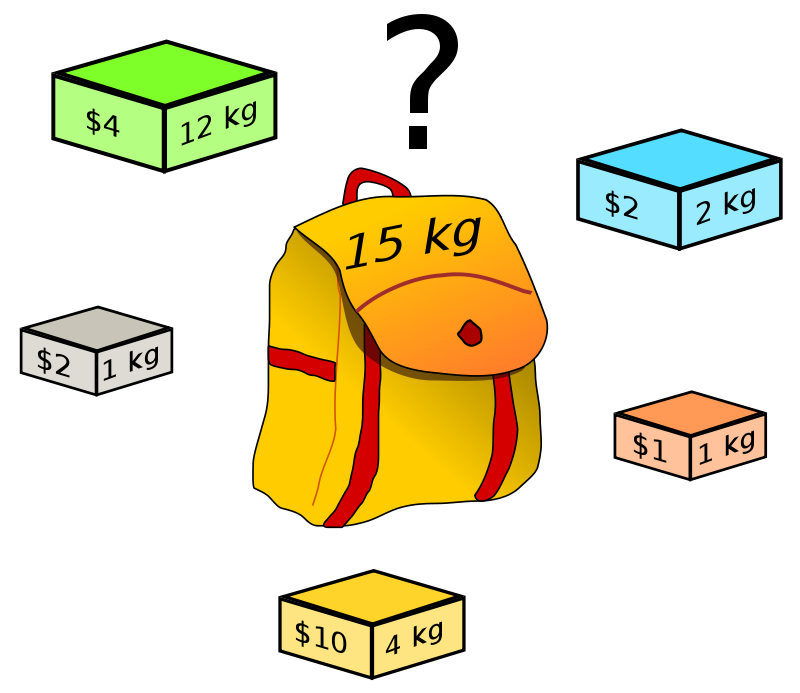
\includegraphics[scale=0.15]{Knapsack.png}
\end{figure}

\end{frame}

\begin{frame}
\frametitle{Sumário}
\tableofcontents
\end{frame}

% CARACTERIZAÇÃO DO PROBLEMA
\section{Caracterização do problema}

\begin{frame}
\frametitle{Definição intuitiva}

    Dado um conjunto de itens, com cada item tendo um peso
    e um custo, qual a escolha de itens tal que a soma de seus pesos é menor
    que a capacidade de uma mochila a soma de seus custos é a maior possível?

\end{frame}

\begin{frame}
\frametitle{Definição matemática: problema de otimização}

    Dados uma mochila com capacidade máxima $W$, um conjunto de $n$ itens $y_{1}, y_{2}, ..., y_{n}$,
    cada um com um peso $w_{i}$ e um valor $v_{i}$:\\

    \begin{equation*}
        \text{maximizar} \sum_{i=1}^{n} v_{i} x_{i}
    \end{equation*}

    \begin{equation*}
        \mbox{sujeito a } \sum_{i=1}^{n} w_{i} x_{i} \leq W \mbox{ e } x_{i} \in \{0,1\}
    \end{equation*}

    Neste caso, $x_{i}$ representa o número de instâncias do item $i$ dentro da mochila.

\end{frame}

\begin{frame}

\frametitle{Problema de otimização: Exemplo}
    Dada uma mochila com capacidade máxima $W = 5$ e dado 4 itens \{$y_{1}, y_{2}, y_{3}, y_{4}$\} com valores \{50, 40, 30, 45\} e com os pesos\\ \{4, 2, 1, 3\}, qual a seleção de itens que possui a maior soma possível de valores com a soma de pesos menor ou igual a 5?

\end{frame}

\begin{frame}
    \frametitle{Definição matemática: problema de decisão}

    Dados uma mochila com capacidade máxima $W$, um valor mínimo $V$, um conjunto de $n$ itens $y_{1}, y_{2}, ..., y_{n}$,
    cada um com um peso $w_{i}$ e um valor $v_{i}$:\\

    \begin{equation*}
        \text{maximizar} \sum_{i=1}^{n} v_{i} x_{i} \text{ t.q.}
    \end{equation*}

    \begin{equation*}
        \begin{split}
            &\quad \sum_{i=1}^{n} w_{i} x_{i} \leq W \mbox{ e } x_{i} \in \{0,1\} \\
            &\quad \sum_{i=1}^{n} v_{i} x_{i} \geq V \mbox{ e } x_{i} \in \{0,1\} \text{ ?}
        \end{split}
    \end{equation*}

    O problema de decisão se torna: "Existe uma seleção de $x_{i}$ que satisfaça essa definição?"

\end{frame}

\begin{frame}
\frametitle{Problema de decisão: Exemplo}
    Dada uma mochila com capacidade máxima $W = 5$ e dado 4 itens \{$y_{1}, y_{2}, y_{3}, y_{4}$\} com valores \{50, 40, 30, 45\} e com os pesos \{4 2 1 3\}, existe uma seleção de itens que possui a soma de seus valores igual ou maior que 85 e a soma de pesos menor ou igual a 5?

\end{frame}

\begin{frame}
    \frametitle{Aplicações}
    \textbf{Estudar na noite de anterior de uma prova:} \\
    Um estudante que tem uma prova no dia seguinte e tem um conjunto
    de capítulos para estudar, cada qual com uma probabilidade de cair
    na prova e um tempo necessário para estudo. Selecionar quais capítulos
    estudar antes da prova é análogo ao problema da mochila binária, e como
    veremos em breve, é \textit{NP-completo}. \\
    
    \textbf{Outros exemplos:} \\
    \begin{itemize}
        \item
            Gerenciadores de download
        \item
            Programas espaciais

    \end{itemize}


\end{frame}

%%%%%%%%%%%%%%%%%%%%%%%%%%%%%%%%%%%%%%%%%%%%%%%%%%%%%%

% PROVA QUE PERTENCE A NP
\section{Problema da mochila binária $\in$ NP}

\subsection{Algoritmo de verificação}
\begin{frame}
    \frametitle{Algoritmo de verificação}
    Para provar que PM\footnotemark $\in$ NP, precisamos mostrar que existe um algoritmo
    capaz de verificar se um certificado do PM é correto em tempo polinomial.

    \footnotetext[1]{PM = Problema da mochila binária}
\end{frame}


\begin{frame}[fragile]
    \frametitle{Algoritmo em pseudocódigo}

    P: conjunto de pesos $p_{i}$ \\
    V: conjunto de valores $v_{i}$ \\
    VMIN: valor minímo para o problema de decisão \\
    W: carga máxima da mochila \\
    n: tamanho do problema \\
    CERTIFICADO: seleção $x_{1},...,x_{n}\ t.q.\ x \in \{0,1\}$ \\

    \begin{block}{Pré-algoritmo}
    \begin{semiverbatim}
    VerificaPM(P, V, VMIN, W, n, CERTIFICADO)
        ...
        returns SIM or NÃO
    \end{semiverbatim}
    \end{block}

\end{frame}

\begin{frame}[fragile]
    \begin{block}{Algoritmo completo}
        \begin{semiverbatim}
        1. VerificaPM(P, V, VMIN, W, n, CERTIFICADO)
        2.    PesoTotal = 0
        3.    ValorTotal = 0
        4.    for i in 1:n
        5.        PesoTotal += CERTIFICADO[i] * P[i]
        6.        ValorTotal += CERTIFICADO[i] * V[i]
        7.    endfor
        8.    if PesoTotal <= W && ValorTotal > VMIN
        9.        return True
        10.    else
        11.       return false
        \end{semiverbatim}
    \end{block}

\end{frame}

\subsection{Análise de complexidade}
\begin{frame}
    \frametitle{Análise de complexidade}

    \begin{itemize}
        \item As atribuições das linhas 2 e 3 tem complexidade $\mathcal{O}(1)$.

        \item O laço $for$ executa $n$ vezes, e a complexidade das atribuições e multiplicações são constantes. Este laço é expresso pelo seguinte somatório:
        \begin{equation*}
            \sum_{i=1}^{n} 2
         \end{equation*}
        A resolução do somatório é dada por $2n$, logo, a complexidade total do laço é $\mathcal{O}(n)$.
        \item o retorno na linha 9 e 11 é constante.
        \item A complexidade total do algoritmo é, portanto, $\mathcal{O}(n)$.
        \item O problema da mochila (como problema de decisão) pode, então, ser verificado em tempo polinomial.
              Com isso concluímos que pertence ao conjunto $NP$.
    \end{itemize}

\end{frame}


% PROVA QUE PERTENCE A NP-DIFICIL
\section{Problema da mochila binária $\in$ NP-difícil}

\subsection{Problema NP-difícil usado}
\begin{frame}
    \frametitle{Soma de subconjuntos}
    \begin{itemize}
        \item
            Para demonstrar que PM $\in$ NP-difícil, utilizaremos uma redução do problema
            da soma de subconjuntos, que já sabemos que é NP-completo, para o problema da mochila.
        \item
            Note que estamos utilizando problemas de decisão, mas se demonstrarmos que
            eles pertencem a NP-difícil, é evidente que o problema de otimização associado
            também será NP-difícil (o problema de decisão é mais "fácil").
    \end{itemize}

\end{frame}

% DEFINICAO SOMA DE SUBCONJUNTOS
\begin{frame}
    \frametitle{Soma de subconjuntos}
        Dado um conjunto de $n$ números inteiros positivos $a_{1}, a_{2}, ..., a_{n}$, e um valor $t \geq 0$ , existe um subconjunto destes números tal que:
         \begin{equation*}
            \sum_{i=1}^{n} a_{i} x_{i} = t \mbox{ e } x_{i} \in \{0,1\}
         \end{equation*}
        $x_{i}$ indica se $a_{i}$ faz parte do subconjunto (1) ou não (0)
        \newline
        \newline
        O problema de decisão é similar ao anterior: "Existe uma seleção de $a_{i}$ que satisfaça essa definição?"
\end{frame}

\begin{frame}
    \frametitle{Soma de subconjuntos: Exemplo}
        Considere o conjunto $A = \{1, 2, 3, 4, 5, 6\}$. Existe um subconjunto tal que a soma de seus elementos é igual a $10$? \\
        Sim! Um exemplo é o subconjunto $A_{1} = \{5, 4, 1\}$. Apesar de existirem outros conjuntos que satisfaçam essa condição, é necessário a existência de pelo menos um para que a resposta para a pergunta seja sim.
\end{frame}

% REDUCAO DAS INSTANCIAS DE A PARA INSTANCIAS DE B
\subsection{Redução PM para SSC}
\begin{frame}
    \frametitle{Redução PM para SSC}
        A redução das instâncias do Problema da Mochila para a Soma de subconjuntos é trivial, já que devemos somar um subconjunto de valores a partir de todo um conjunto em ambos os casos.
        \newline
        \newline
        Para todos os $n$ elementos $a_{1}, a_{2}, ..., a_{n}$ fazemos a seguinte transformação:
        \begin{equation*}
            w_{i} = a_{i}
        \end{equation*}
        \begin{equation*}
            v_{i} = a_{i}
        \end{equation*}
        Para a capacidade máxima $W$ e o valor mínimo $V$, fazemos a seguinte transformação:
        \begin{equation*}
            W = t
        \end{equation*}
        \begin{equation*}
            V = t
        \end{equation*}
        
\end{frame}

\begin{frame}
    \frametitle{Redução PM para SSC}
        Com isso, conseguimos mapear as exatas mesmas respostas do problema de decisão da Soma de subconjuntos para o problema de decisão da Mochila.
         \begin{equation*}
            \sum_{i=1}^{n} w_{i} x_{i} \leq W \mbox{ terá as mesmas respostas (sim ou não) que } \sum_{i=1}^{n} a_{i} x_{i} = t
         \end{equation*}
         \begin{equation*}
            \sum_{i=1}^{n} v_{i} x_{i} \geq V \mbox{ terá as mesmas respostas (sim ou não) que } \sum_{i=1}^{n} a_{i} x_{i} = t
         \end{equation*}
\end{frame}

% EXEMPLO DE REDUÇÃO
\begin{frame}
    \frametitle{Redução PM para SSC: Exemplo}
        Considerando o conjunto $a = \{2, 3, 5, 7, 10\}$ e um valor $t = 17$, a redução se dá da seguinte forma:
        \begin{equation*}
            w_{i} = a_{i} \longrightarrow w = \{2, 3, 5, 7, 10\}
        \end{equation*}
        \begin{equation*}
            v_{i} = a_{i} \longrightarrow v = \{2, 3, 5, 7, 10\}
        \end{equation*}
        \begin{equation*}
            W = t \longrightarrow W = 17
        \end{equation*}
        \begin{equation*}
            V = t \longrightarrow V = 17
         \end{equation*}
\end{frame}

\begin{frame}
    \frametitle{Redução PM para SSC: Exemplo}
        O problema da SSC, com o conjunto $a = \{2, 3, 5, 7, 10\}$ e um valor $t = 17$ possui solução.
        Uma solução válida é o subconjunto \{2, 3, 5, 7\}.\\
        Após a redução, temos que este mesmo subconjunto é também uma solução válida para o Problema da Mochila:
        \begin{equation*}
            \mbox{Peso máximo da mochila: } 2 + 3 + 5 + 7 \leq W = 17
        \end{equation*}
        \begin{equation*}
            \mbox{Valor mínimo da mochila: } 2 + 3 + 5 + 7 \geq V = 17
        \end{equation*}

\end{frame}

% ALGORITMO DE REDUCAO
\subsection{Algoritmo de redução}
\begin{frame}[fragile]
\frametitle{Algoritmo de redução}
    n: tamanho do problema \\
    t: soma total formada por um subconjunto dos valores $a_{i}$ \\
    a: vetor com os valores $a_{i}$ \\
    \begin{block}{Algoritmo de Redução}
        \begin{semiverbatim}
        1. ReducaoSSCparaPM(n, t, a)
        2.    W = t
        3.    V = t
        4.    for i in 1:n
        5.        w[i] = a[i]
        6.        v[i] = a[i]
        7.    endfor
        8.    return n, w, v, W, V
        \end{semiverbatim}
    \end{block}
\end{frame}


% ANALISE DA COMPLEXIDADE
\subsection{Análise da complexidade}
\begin{frame}
\frametitle{Análise da complexidade}
    \begin{itemize}
        \item As atribuições das linhas 2 e 3 tem complexidade $\mathcal{O}(1)$.

        \item Nas linhas 4 a 7, o laço $for$ executa $n$ vezes com duas atribuições que são constantes. Isso é expresso pelo seguinte somatório
         \begin{equation*}
            \sum_{i=1}^{n} 2
         \end{equation*}
        A resolução do somatório é dada por $2n$, logo, a complexidade total do laço é $\mathcal{O}(n)$.
        \item O retorno na linha 8 tem a complexidade $\mathcal{O}(1)$.
        \item A complexidade total do algoritmo é, portanto, $\mathcal{O}(n)$.
        \item Como a complexidade da redução está dentro do tempo polinomial, provamos que o Problema da Mochila $\in$ NP-difícil.
    \end{itemize}
\end{frame}

\begin{frame}
\frametitle{NP-completude do Problema da Mochila}
    \begin{itemize}
        \item Foi provado que existe um algoritmo de verificação para o Problema da Mochila em tempo polinomial, logo, temos que o Problema da Mochila $\in$ NP.
        \item Foi provado também que existe uma redução em tempo polinomial do problema da Soma de Subconjuntos para o Problema da Mochila, logo, temos também que o Problema da Mochila $\in$ NP-difícil.
        \item Com isso, concluímos que o Problema da Mochila $\in$ NP-completo.
    \end{itemize}
\end{frame}
\end{document}


% TODO:
% exemplos dos problemas e otimização e decisão (feito)
% somatórios na análise de complexidade (feito)
% exemplos de redução (feito)
